\documentclass{scrartcl}

\usepackage{amssymb}
\usepackage{amsmath}
\usepackage{tikz}
\usetikzlibrary{calc}						%for centerarc
\usetikzlibrary{decorations.pathreplacing}	%for brackets

\def\centerarc[#1](#2)(#3:#4:#5)% Syntax: [draw options] (center) (initial angle:final angle:radius)
{ \draw[#1] ($(#2)+({#5*cos(#3)},{#5*sin(#3)})$) arc (#3:#4:#5); }

%from Baudouin, Charles. (1970). De l'instinct à l'esprit. Neuchâtel: Delachaux et Niestlé, p. 224

\begin{document}
	
	\hspace{-2cm}%
	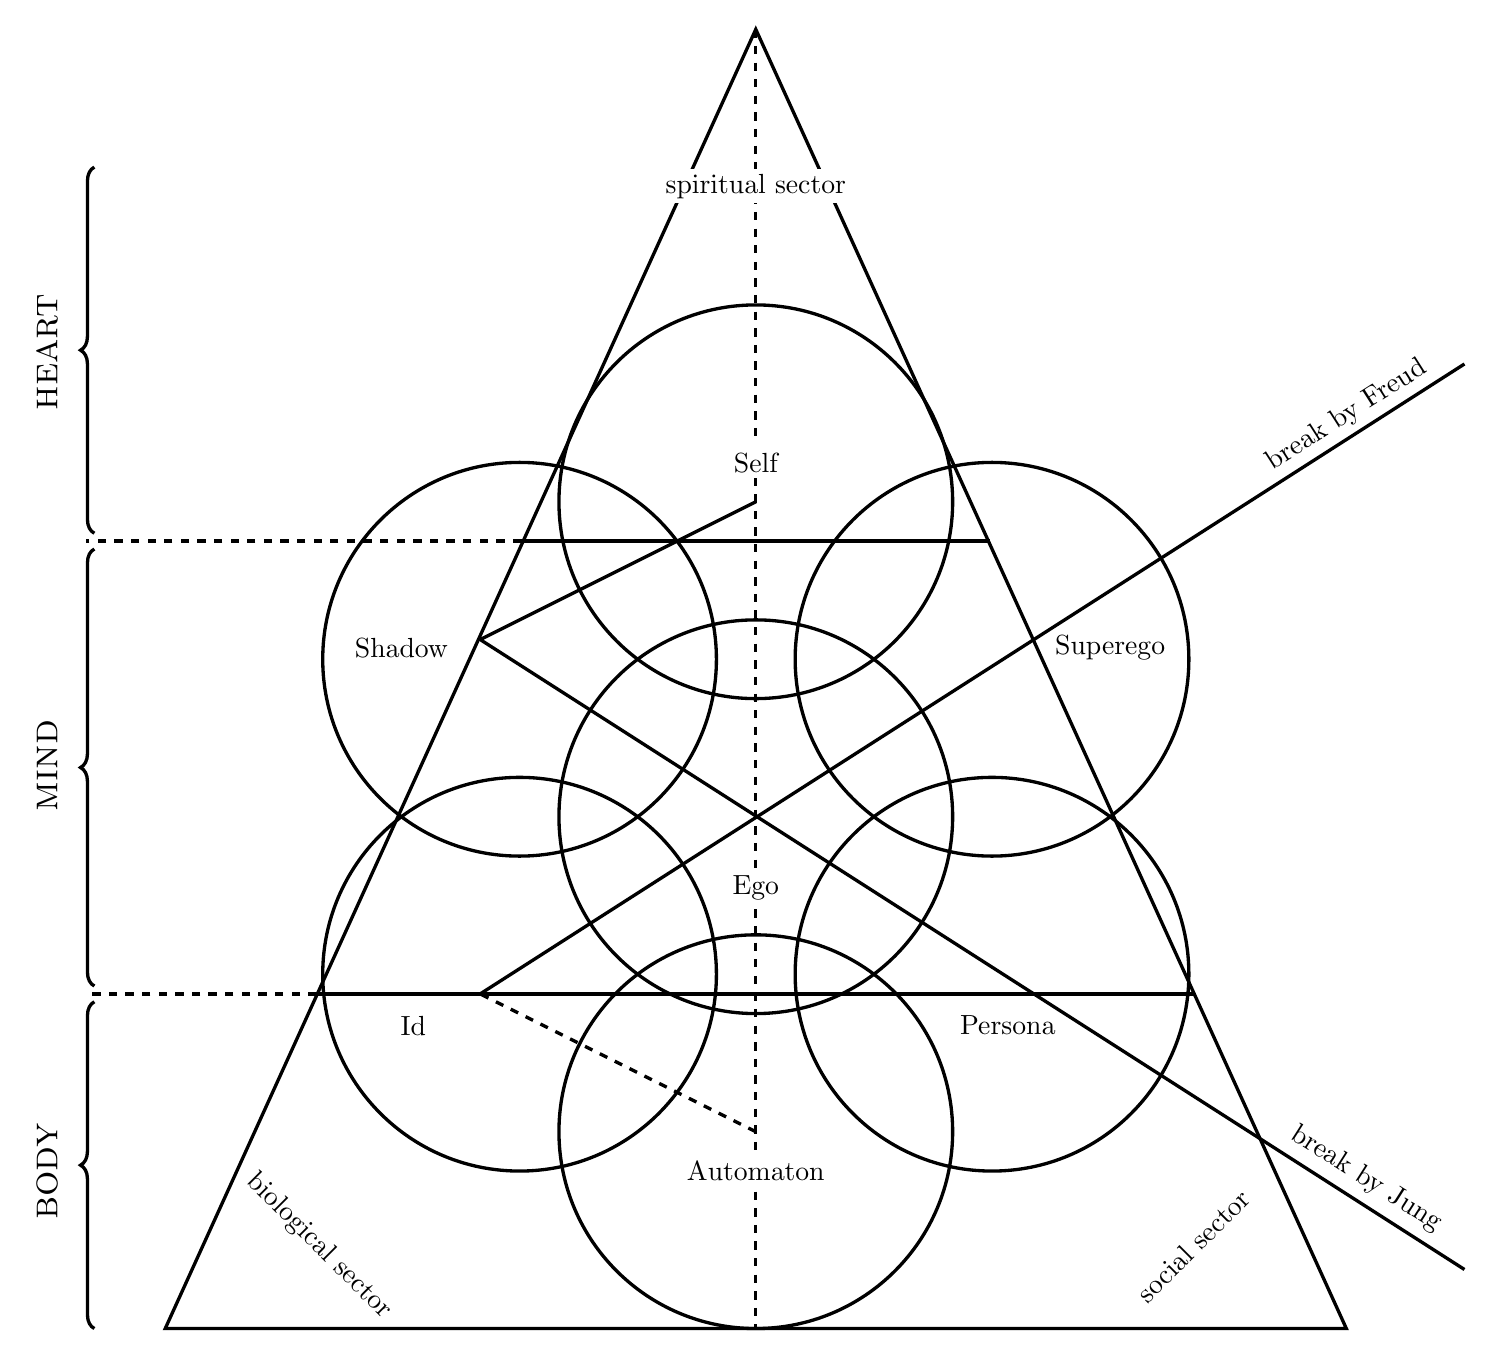
\begin{tikzpicture}[very thick]	
	%CIRCLES
	\centerarc[dashed,<->,>=latex](0,0)(32.5:150:7.5)
	\centerarc[dashed,<->,>=latex](0,0)(150:270:7.5)
	\centerarc[dashed,<->,>=latex](0,0)(-90:32.5:7.5)
	%\draw[dashed] (0,0) circle (7.5cm);
	\draw (0,4) circle (2.5cm);		%top circle
	\draw (-3,2) circle (2.5cm);	%top left
	\draw (-3,-2) circle (2.5cm);	%low left
	\draw (0,0) circle (2.5cm);		%mid circle
	\draw (3,2) circle (2.5cm);		%top right
	\draw (3,-2) circle (2.5cm);	%low right
	\draw (0,-4) circle (2.5cm);	%low circle
		
	%TRIANGLE
	\draw (-7.5,-6.5)--(0,10)--(7.5,-6.5)--cycle;
	\draw[dashed] (0,10)--(0,-6.5);					%vertical line
	\draw (-2.98,3.5)--(2.98,3.5);					%top horizontal line
		\draw[dashed] (-2.98,3.5)--(-8.5,3.5);
	\draw (-5.58,-2.25)--(5.58,-2.25);				%low horizontal line
		\draw[dashed] (-5.58,-2.25)--(-8.5,-2.25);
	
	%DIAGONAL LINES
	\draw (0,4)--(-3.5,2.25)--(9,-5.75);	%coupe selon Jung
	\draw[dashed] (0,-4)--(-3.5,-2.25);		%coupe selon Freud
	\draw (-3.5,-2.25)--(9,5.75);
	
	%LABELS
%	\node at (0,0) {};
		\fill[white] (-0.4,4.3) rectangle (0.4,4.8);
	\node at (0,4.5)		{Self};
	\node at (-4.5,2.15)	{Shadow};
	\node at (4.5,2.15)		{Superego};
		\fill[white] (-0.3,-0.7) rectangle (0.3,-1.1);
	\node at (0,-0.9)		{Ego};
	\node at (-4.35,-2.65)	{Id};
	\node at (3.2,-2.65)	{Persona};
		\fill[white] (-1,-4.3) rectangle (1,-4.75);
	\node at (0,-4.5)		{Automaton};
	%
	\node at (7.5,5.1)		{\rotatebox{32.5}{break by Freud}};
	\node at (7.75,-4.6)	{\rotatebox{-32.5}{break by Jung}};
	%
		\fill[white] (-1.25,7.8) rectangle (1.25,8.23);
	\node at (0,8)			{spiritual sector};
	\node at (-5.55,-5.45)	{\rotatebox{-45}{biological sector}};
	\node at (5.55,-5.45)	{\rotatebox{45}{social sector}};
	%
	\draw[decorate,decoration={brace,amplitude=5pt},yshift=0pt] (-8.4,3.6)--(-8.4,8.25);	%top bracket
	\draw[decorate,decoration={brace,amplitude=5pt},yshift=0pt] (-8.4,-2.15)--(-8.4,3.4);	%mid bracket
	\draw[decorate,decoration={brace,amplitude=5pt},yshift=0pt] (-8.4,-6.5)--(-8.4,-2.35);	%low bracket
	%
	\node at (-9,5.9)	{\rotatebox{90}{\Large\textsc{heart}}};
	\node at (-9,0.65)	{\rotatebox{90}{\Large\textsc{mind}}};
	\node at (-9,-4.5)	{\rotatebox{90}{\Large\textsc{body}}};
	
	%\draw[help lines] (-5,-5) grid (5,5);
	\end{tikzpicture}
	
\end{document}